%%%%%%%%%%%%%%%%%%%%%%%%%%%%%%%%%%%%%%%%%%%%%%%%%%%%%%%%%%%%%%%%%%%%%%%%%%%%%%%%
\documentclass[twocolumn]{revtex4}

%%%%%%%%%%%%%%%%%%%%%%%%%%%%%%%%%%%%%%%%%%%%%%%%%%%%%%%%%%%%%%%%%%%%%%%%%%%%%%%%
% Note that comments begin with a "%" and are not turned into text in the .pdf
% document.
%%%%%%%%%%%%%%%%%%%%%%%%%%%%%%%%%%%%%%%%%%%%%%%%%%%%%%%%%%%%%%%%%%%%%%%%%%%%%%%%

%%%%%%%%%%%%%%%%%%%%%%%%%%%%%%%%%%%%%%%%%%%%%%%%%%%%%%%%%%%%%%%%%%%%%%%%%%%%%%%%
% Include some extra packages.
%%%%%%%%%%%%%%%%%%%%%%%%%%%%%%%%%%%%%%%%%%%%%%%%%%%%%%%%%%%%%%%%%%%%%%%%%%%%%%%%
\usepackage[]{graphicx}
%%%%%%%%%%%%%%%%%%%%%%%%%%%%%%%%%%%%%%%%%%%%%%%%%%%%%%%%%%%%%%%%%%%%%%%%%%%%%%%%

%%%%%%%%%%%%%%%%%%%%%%%%%%%%%%%%%%%%%%%%%%%%%%%%%%%%%%%%%%%%%%%%%%%%%%%%%%%%%%%%
\begin{document}

%%%%%%%%%%%%%%%%%%%%%%%%%%%%%%%%%%%%%%%%%%%%%%%%%%%%%%%%%%%%%%%%%%%%%%%%%%%%%%%%
\title{
Software Final
}

\author{D.~Finnegan}

\affiliation{Siena College, Loudonville, NY}

\date{\today}

\begin{abstract}
	The purpose of this assignment is to test our knowledge and skills with the coding tools Python, Latex, and Git. Since there are so many different tools being used, there are many different parts to the project. The first part involves using Python to figure out where and when the raptor and human meet, which came out to be after two seconds at 36 meters. Then finding the probability that the human will escape. This was found to be around sixty to sixty five percent.  	
\end{abstract}

\maketitle

\section{Introduction}
In this project, I was given the average speed of a human and the average speed of a velociraptor. Using these two pieces of information, I had to use the coding tool Python to solve whether or not a person would escape a velociraptor chasing after them if they had a thirty meter head start. To do this I had to use much of what I have learned throughout this semester to write the code that would figure all this out along with making a few plots that help visualize the scenario and when if the person will survive or not. 
\section{Problem One: Position vs Time}
	In this problem I had to generate a position versus time plot showing both the velociraptor and humans progress running each second. Before I started anything for the code, I set variables for both the raptor and human equal to their respective beginning positions along with separate variables for each of their average speeds. Then I set "t" or the "time" equal to a range of numbers between zero and one thousand. Using that, I then took those numbers and plugged each of the numbers in the list of t, the i's, and divided each one by the integer 100.0 to create a range going up to 10 that was filled with smaller, more precise numbers. After creating my numbers for time, I used them, along with my variables i set earlier, to create two separate lists of numbers that would be the distance they traveled each second. To do this i set a variable "xr" and "xh", the distance traveled by the raptor and then human, both equal to empty brackets. These empty brackets act as an empty list. This is needed because in my code to get the distance each of them have gone since the start by each second, I have to make a loop that uses the physics kinematics equation $ x_f = x_0 + v_0 t$ and adds/appends the number created to that empty list. Once I created all of these lists for both the raptor and human, all i had to do afterwards was use the imported matplotlib tools to plot the time "t" against their positions "xh" and "xr".  
\begin{figure}[h]
	\centering
	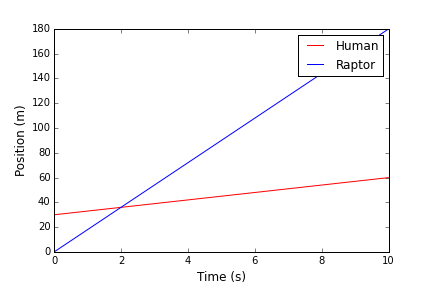
\includegraphics[width=.5\textwidth]{RaptorvHuman_Finnegan.png}
	\caption{Position vs Time plot \label{fig:Position vs Time plot}}
\end{figure}

\section{Problem Two: When does 'raptor catch up to you?}
 	For the next problem I had to use what I plotted in problem one to find the distance they both traveled until the 'raptor is right next to the human. To do this i created a loop that first took each number from from the list "t" and made them back into integers by multiplying them by 100. Before i did this each of the numbers in "t" went up by .01, and so to get them back to 1, 2, 3, and so on i multiplied them all by 100. Now having these new numbers of time, I used an if statement to have the loop go over every point in both position lists and compare the two to see when their positions were equal. By making this an if statement, I made it so that once it found where they were at equal positions it would print their position and time. To find the position, it plugged in two seconds first, and then after being multiplied by 100, it compared the 200th spot in each of the position lists. This then find that they meet at 36 meters after 2 seconds.

\section{Problem Three: When is it close enough to strike?}
	For this next problem, I went about solving it almost the same way as the last problem, except I had to make some minor changes so that instead of showing when they are at the same position, it would show when the 'raptor is about one meter behind the human. Using the same code from the last problem, I changed the if statement so that it would again look over and compare each of the lists of positions of both the human and raptor, but this time I set it up so that it would fine the points when the position of the human subtracted by the position of the raptor equaled one. Then in the same if statement i set it up so that it would stop going through the rest of the numbers, or break, once it found the point where the raptor is about one meter behind the human. After this I copied the same plot as the one from problem one over to this problem but added an arrow using the "plt" command for arrow to place it at the point. Once you run it the solution comes out as the raptor is 1 meter behind the human after on 1.94 seconds and the human has only ran 5.82 meters.
\begin{figure}[h]
	\centering
	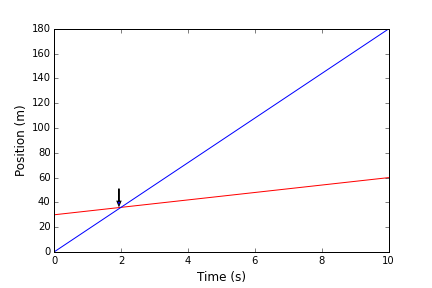
\includegraphics[width=.5\textwidth]{RaptorvHuman_Finnegan_arrow.png}
	\caption{Position vs Time plot with arrow \label{fig: Position vs Time plot}}
\end{figure}

\section{Problem Four: Will it bite you?}
	After figuring out those numbers in problem three, I had to use the same information to solve this next problem. In this problem I had to figure out roughly how good the humans chances are of escaping from the raptor. When the raptor gets to one meter behind the human, it starts to try and bit them. The first time it tries to do so, it has a 20 percent chance of getting you, then after that it drops to 15, then 7 percent since each time it gets frustrated. Using that information i set up a function called raptor and in it i first set three variables called bite1, bite2, and bite3, equal to the sum of 100 random integers. Then i used the conditionals if, elif, and else, to have the code look through the three bites and see if the first one was under twenty, then if the second was under fifteen, if the third was under seven, and finally, if all three were not true then that means the human survived. If one of the three is true then that means the raptor got the human and they are dead. For the bottom half, i set up another for loop with a range that had a thousand numbers inside it. Inside the loop I set the variable gotbit equal to my function above. Then i set up the if conditionals so that each time it went through the function and got an outcome of either "Dead" or "Live" it would add one to the variables for "die" or "live". And since the range goes to a thousand numbers, it will do this one thousand times. After finishing this it takes the number from "live" and divides it by the float one thousand and then multiplies that by one hundred to move the decimal places over and make it a percentage. 
	

\end{document}

























